\chapter{Results and Conclusions}
\label{ch:results}
At the onset of this project, the goal was to simulate, optimize, design, construct, install and run the Radial Time Projection Chamber (RTPC) for the Barely-Offshell Nucleon Structure experiment at 12 GeV (BONuS12). BONuS12 ran successfully from January to March 2020, collecting 3.9 billion triggers and about 2.8 billion triggers with the RTPC. The run was cut short by the COVID19 pandemic, with only half of the expected data collected. Because it was always known that data collection would not be done in time for a full BONuS12 analysis in this work, important analysis on the first experiment (Run Group A) of CLAS12 was done to contribute to data analysis for the collaboration. This chapter will summarize the results of the RGA data analysis as well as the first monitoring and preliminary analysis plots from BONuS12.

\section{RGA Cross Section}
The inclusive deep inelastic scattering differential cross section was extracted for $0.06 < x < 0.74$ and $0.3< y < 0.74$ using data from Run Group A (RGA) Run 5036 (as shown in Fig. \ref{fig:rga_xsec_plots}). The cross section was plotted and compared to the calculated cross section parameterized from fits of $F_1$ and $F_2$ (Eq. \ref{eq:dis_xsec}) by Christy-Bosted.\cite{christy_bosted} Fig. \ref{fig:rga_xsec_plots} shows the inclusive DIS differential cross section (on the y-axis) for the various $y$ bins as a function of Bjorken-$x$ (on the x-axis). The open dots are the extracted cross sections from the RGA data. The green band represents the fit including uncertainty of the DIS cross section calculated from the Christy-Bosted fits to $F_1$ and $F_2$,\cite{christy_bosted} The extracted cross section from RGA data is in reasonable agreement with the model and only begins to differ drastically at lower $x$.

\begin{figure}[h!]
	\centering
	\begin{subfigure}[b]{0.38\linewidth}
		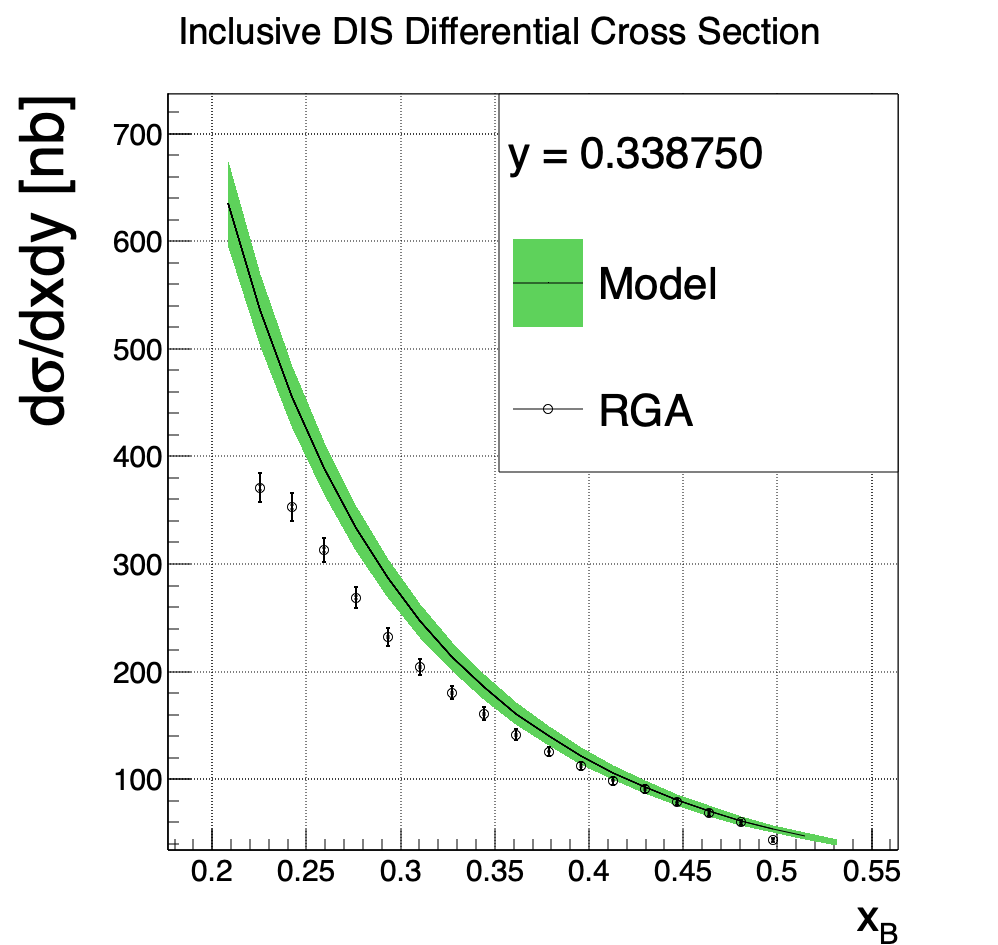
\includegraphics[width=\linewidth]{figures/rga/xsec_0.png}
		\label{fig:rga_xsec0}
	\end{subfigure}
	\begin{subfigure}[b]{0.38\textwidth}
		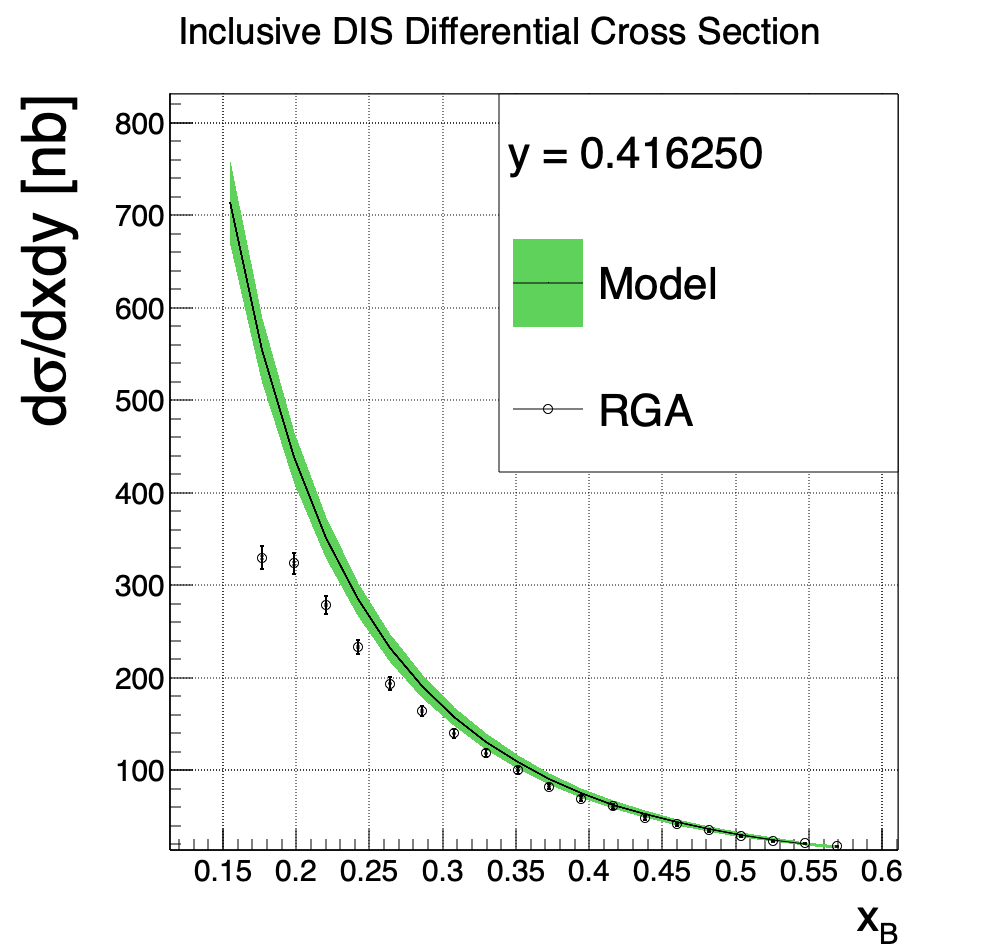
\includegraphics[width=\linewidth]{figures/rga/xsec_1.png}
		\label{fig:rga_xsec1}
	\end{subfigure}
\end{figure}
\begin{figure}[h!]
	\centering
	\begin{subfigure}[b]{0.38\linewidth}
		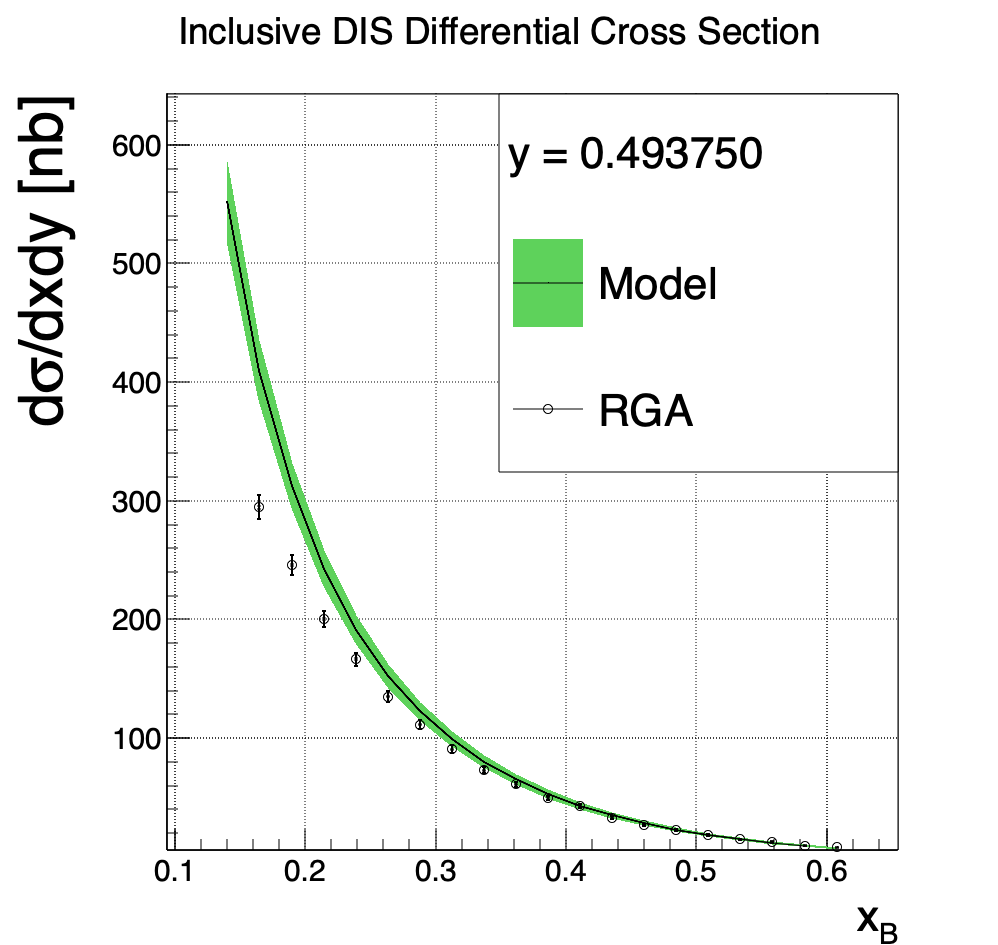
\includegraphics[width=\linewidth]{figures/rga/xsec_2.png}
		\label{fig:rga_xsec2}
	\end{subfigure}
	\begin{subfigure}[b]{0.38\textwidth}
		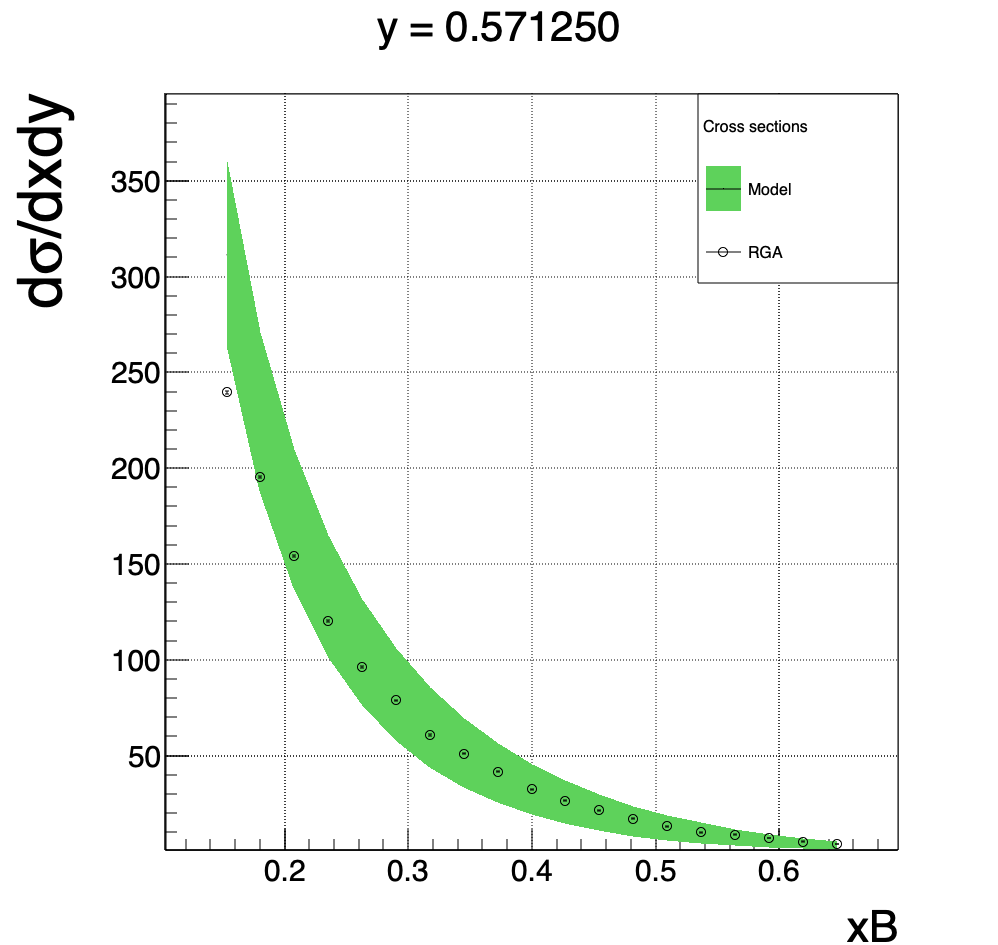
\includegraphics[width=\linewidth]{figures/rga/xsec_3.png}
		\label{fig:rga_xsec3}
	\end{subfigure}
\end{figure}
\begin{figure}[h!]
	\centering
	\begin{subfigure}[b]{0.38\linewidth}
		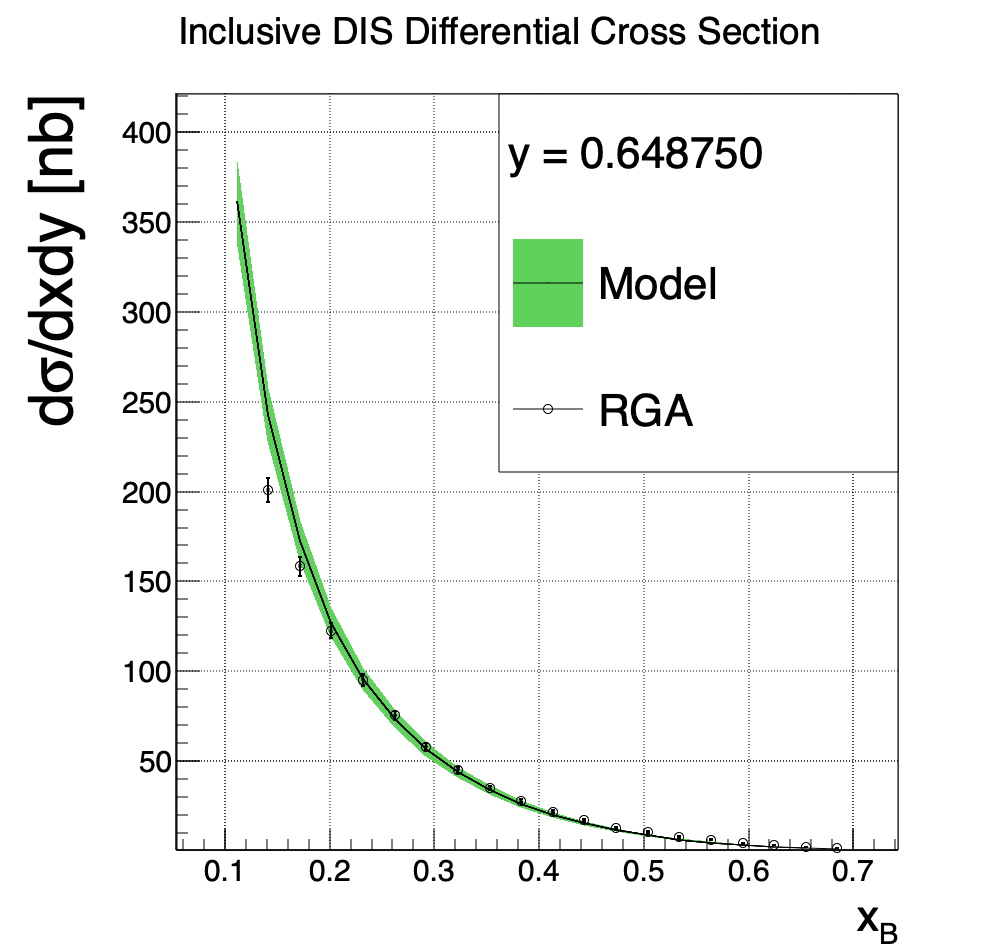
\includegraphics[width=\linewidth]{figures/rga/xsec_4.png}
		\label{fig:rga_xsec4}
	\end{subfigure}
	\begin{subfigure}[b]{0.38\textwidth}
		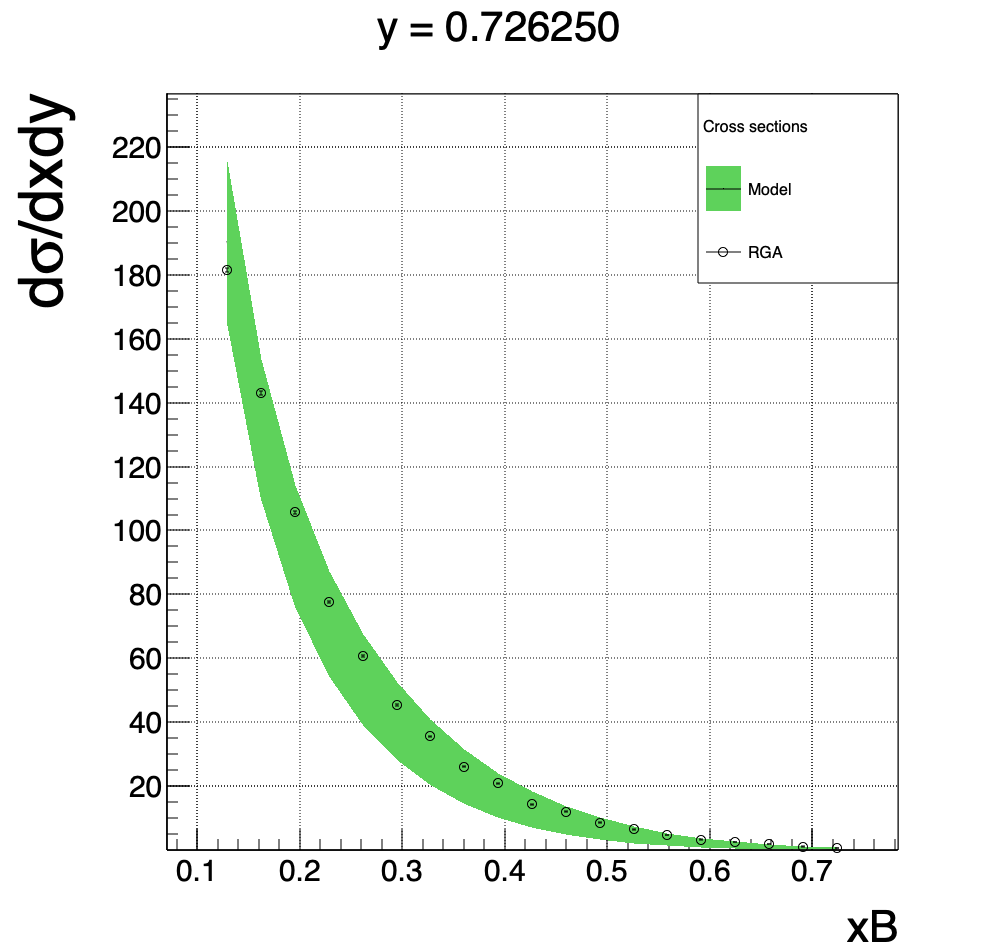
\includegraphics[width=\linewidth]{figures/rga/xsec_5.png}
		\label{fig:rga_xsec5}
	\end{subfigure}
	\caption{Plots of inclusive DIS differential cross section vs $x_B$ for various values of $y$. The green band represents the uncertainty of the DIS cross section calculated from the Christy-Bosted fits to $F_1$ and $F_2$ \cite{christy_bosted}.}
	\label{fig:rga_xsec_plots}
\end{figure}

\cleardoublepage
\section{BONuS12}
During the run time of BONuS12, some adjustment were made and target gases were used. The target was changed from hydrogen H$_2$ to helium $^3$He for calibration and deuterium D$_2$ for production. At the beginning of Run Group F, of which BONuS12 was a part, the beam energy was set to 1 pass around the accelerator to produce 2.14 GeV energy. This allowed the gathering of data to measure elastic scattering from protons in hydrogen, a well known process used to confirm that all detectors were functioning well.  Once the 2.14 GeV data were gathered, the energy was increased to 5 passes to created 10.4 GeV beam electrons.

Once the 10.4 GeV beam energy was reached, it became clear that the RTPC was not operating up to expectations. The number of hits/track and the mean ADC value of those individual hits began to decrease. In order to fix these problems, the potential in the drift region as well the potential differences between each GEM foil was adjusted. The hits/track and mean ADC of the hits would increase for a time (about 6-12 hours), and then those values would decrease again. The magnitude of the magnetic field created by the solenoid was also adjusted. The first runs were at 5T field, and then decreased to 4T. This was in an attempt to decrease the drift angle of the drift electrons, thinking that those electrons were having a difficult time passing through the GEM foils. In all, the first RTPC (RTPC1) was in use for 33 days at roughly 50\% efficiency. After that time, RTPC1 was replaced with another, previously constructed, RTPC (RTPC3) during a 5 day replacement period. RTPC3 ran for 3 days before the shutdown.

\subsection{DMS}
During the running of BONuS12, the RTPC gas system ensured that the proper gas flow rate and pressure was maintained. Downstream of the RTPC, the drift gas flowed through the Drift-gas Monitoring System (DMS). The DMS was there to monitor any fluctuations in important gas properties ($e.g$ temperature, pressure, gas mixture, etc.). The output of the DMS was two TDC readings accumulated in histograms for each channel. Channel 1 (CH1) was the TDC readout for the time difference between the anode signal and the signal from the PMT near to the anode. Channel 2 (CH2) was the TDC readout for the time difference between the anode signal and the signal from the PMT far from the anode.

\begin{figure}[h!]
	\centering
	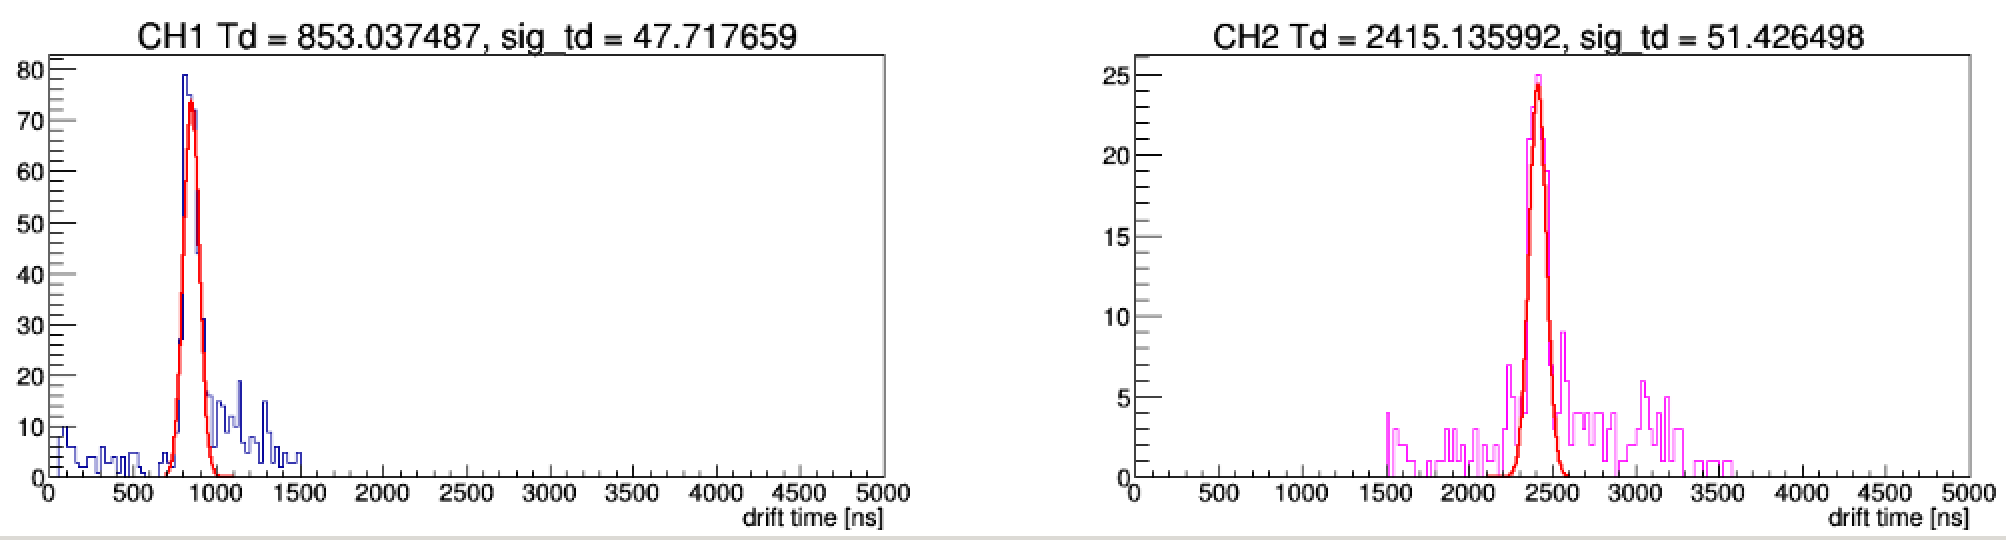
\includegraphics[width=0.99\linewidth]{figures/DMS_11953_time.png}
	\caption{DMS drift time histograms for CH1 (left) and CH2 (right) on Run 11953.}
	\label{fig:dms_11953_time}
\end{figure}
\begin{figure}[h!]
	\centering
	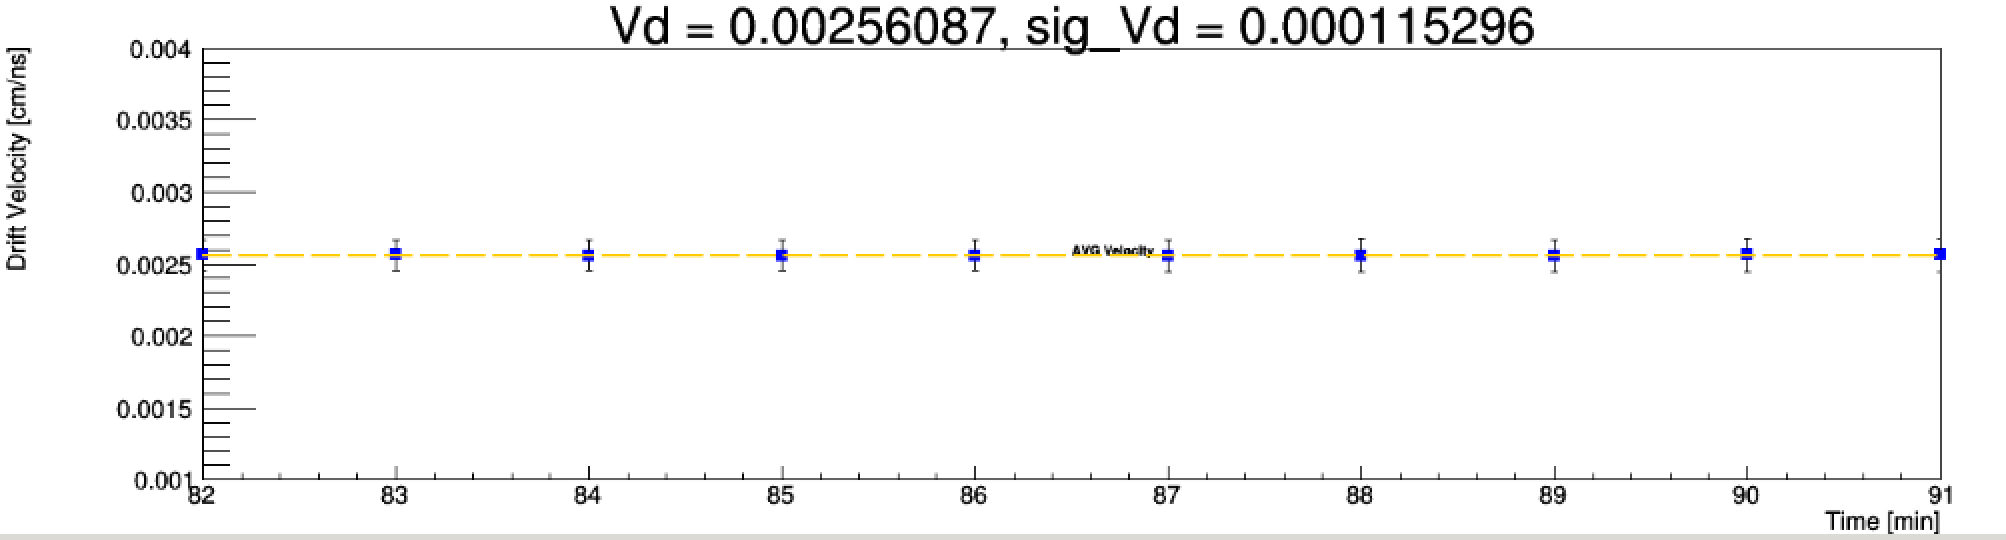
\includegraphics[width=0.99\linewidth]{figures/DMS_11953_velocity.png}
	\caption{DMS drift velocity vs. time graph during Run 11953.}
	\label{fig:dms_11953_velocity}
\end{figure}

Fig. \ref{fig:dms_11953_time} shows an example of the drift time output for channels 1 and 2 (left and right, respectively) for Run 11953. The drift velocity is calculated by
\begin{equation}
v = \frac{\Delta d}{\Delta t} = \frac{4 \; \mathrm{ cm}}{t_{\mathrm{CH2}} - t_{\mathrm{CH1}}}.
\end{equation}
Fig. \ref{fig:dms_11953_velocity} shows the drift velocity vs. time graph for Run 11953. The orange dotted line is the average velocity for the 10 minutes shown on the plot. These plots were indicative of the majority of runs, showing that the gas parameters were relatively stable. The few exceptions occurred for two reasons. 

The first reason for deviations from typical DMS output was its sensitivity to the flow rate of the drift gas through the RTPC. If it was too low, not enough gas would flow into the DMS and the number of accumulated statistics would decrease and the peaks in drift time typical of runs (as in Fig. \ref{fig:dms_11953_time}) would not appear. This did serve as an advantage when identifying empty gas bottles, however. If the flow rate was high and statistics still dropped, it was an indicator that the bottle of drift gas needed to be replaced.

\begin{figure}[h!]
	\centering
	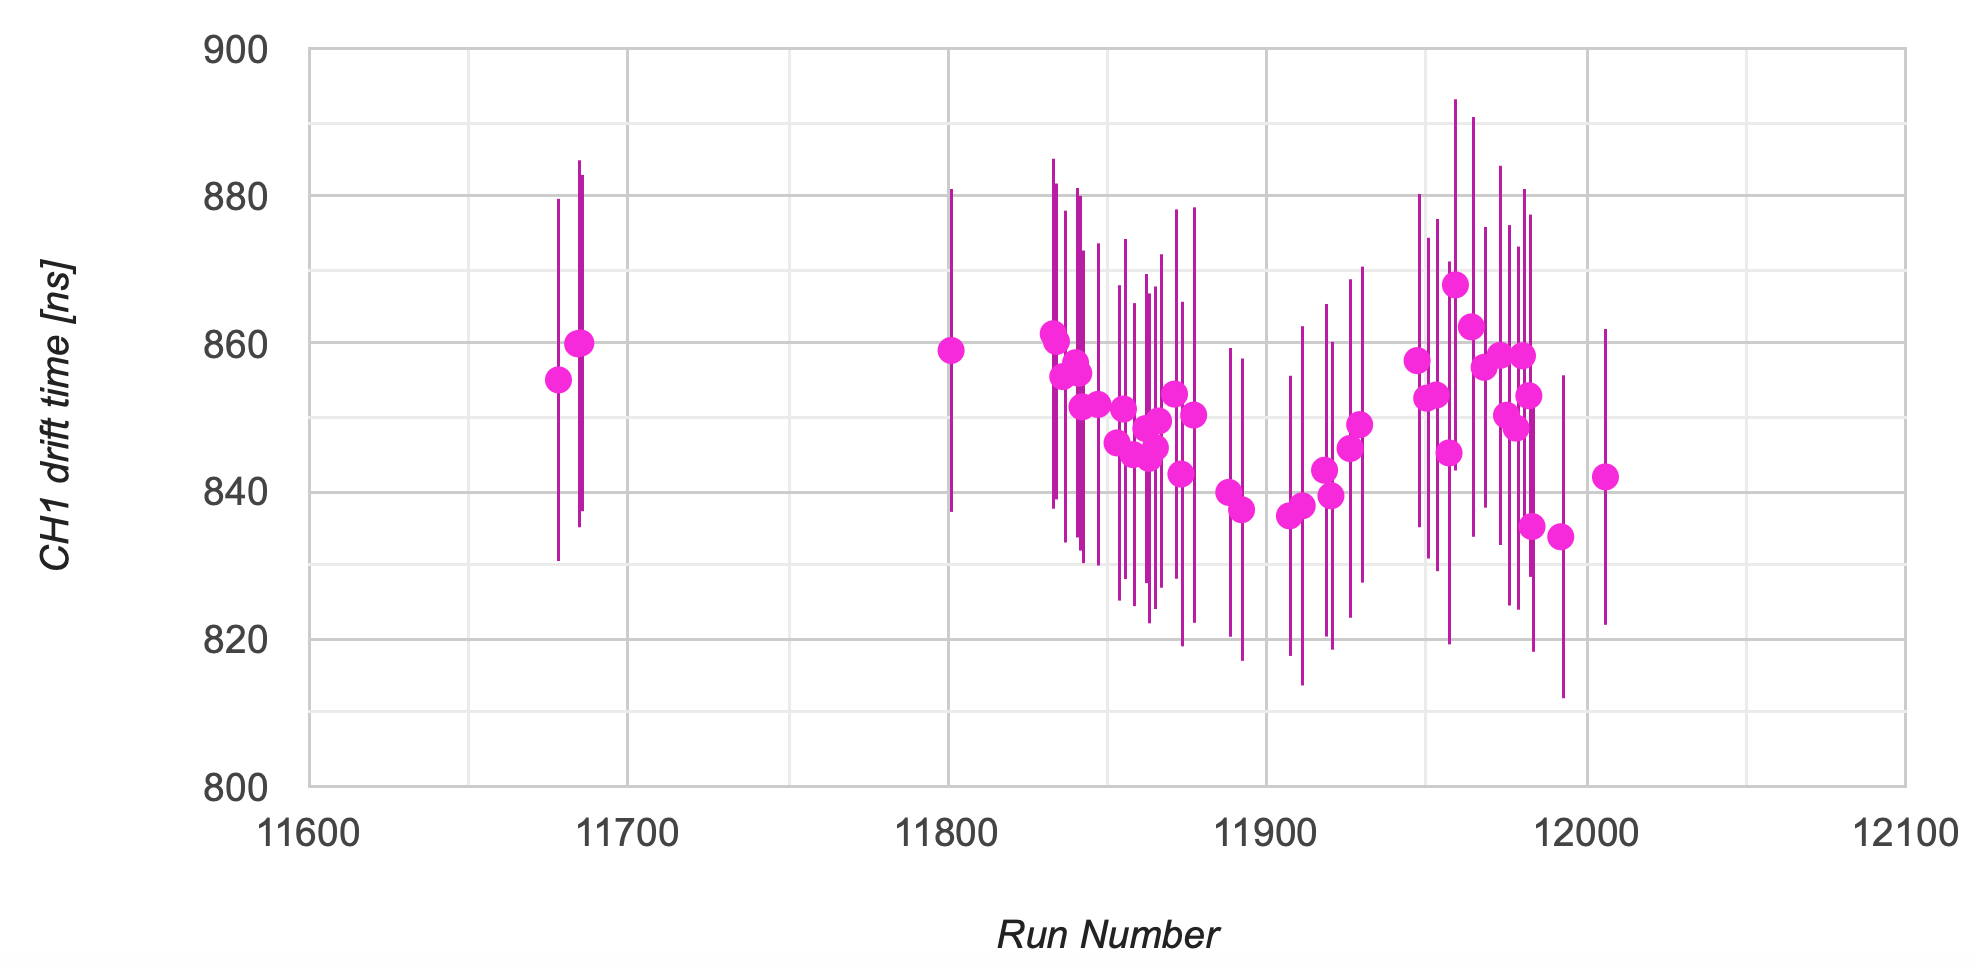
\includegraphics[width=0.9\linewidth]{figures/DMS_ch1_run.png}
	\caption{DMS drift velocity for channel 1 vs. run.}
	\label{fig:dms_ch1_run}
\end{figure}
\begin{figure}[h!]
	\centering
	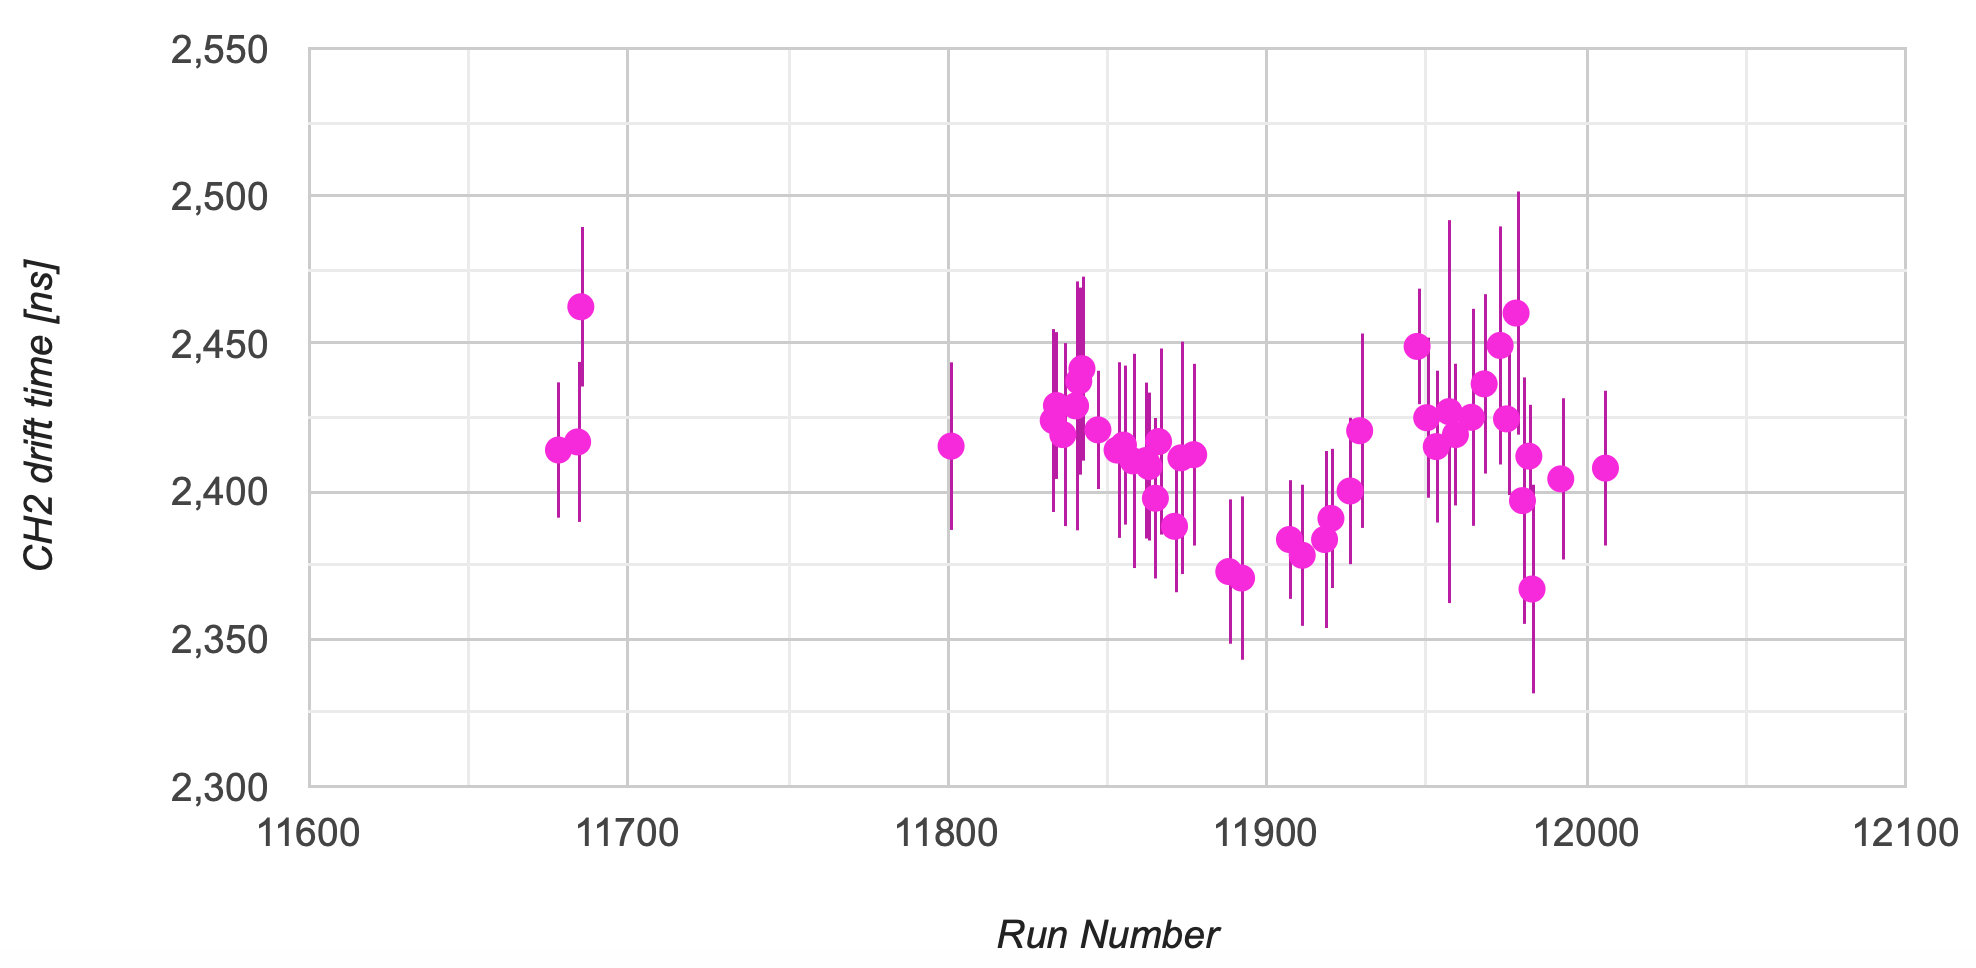
\includegraphics[width=0.9\linewidth]{figures/DMS_ch2_run.png}
	\caption{DMS drift velocity for channel 2 vs. run.}
	\label{fig:dms_ch2_run}
\end{figure}
\begin{figure}[h!]
	\centering
	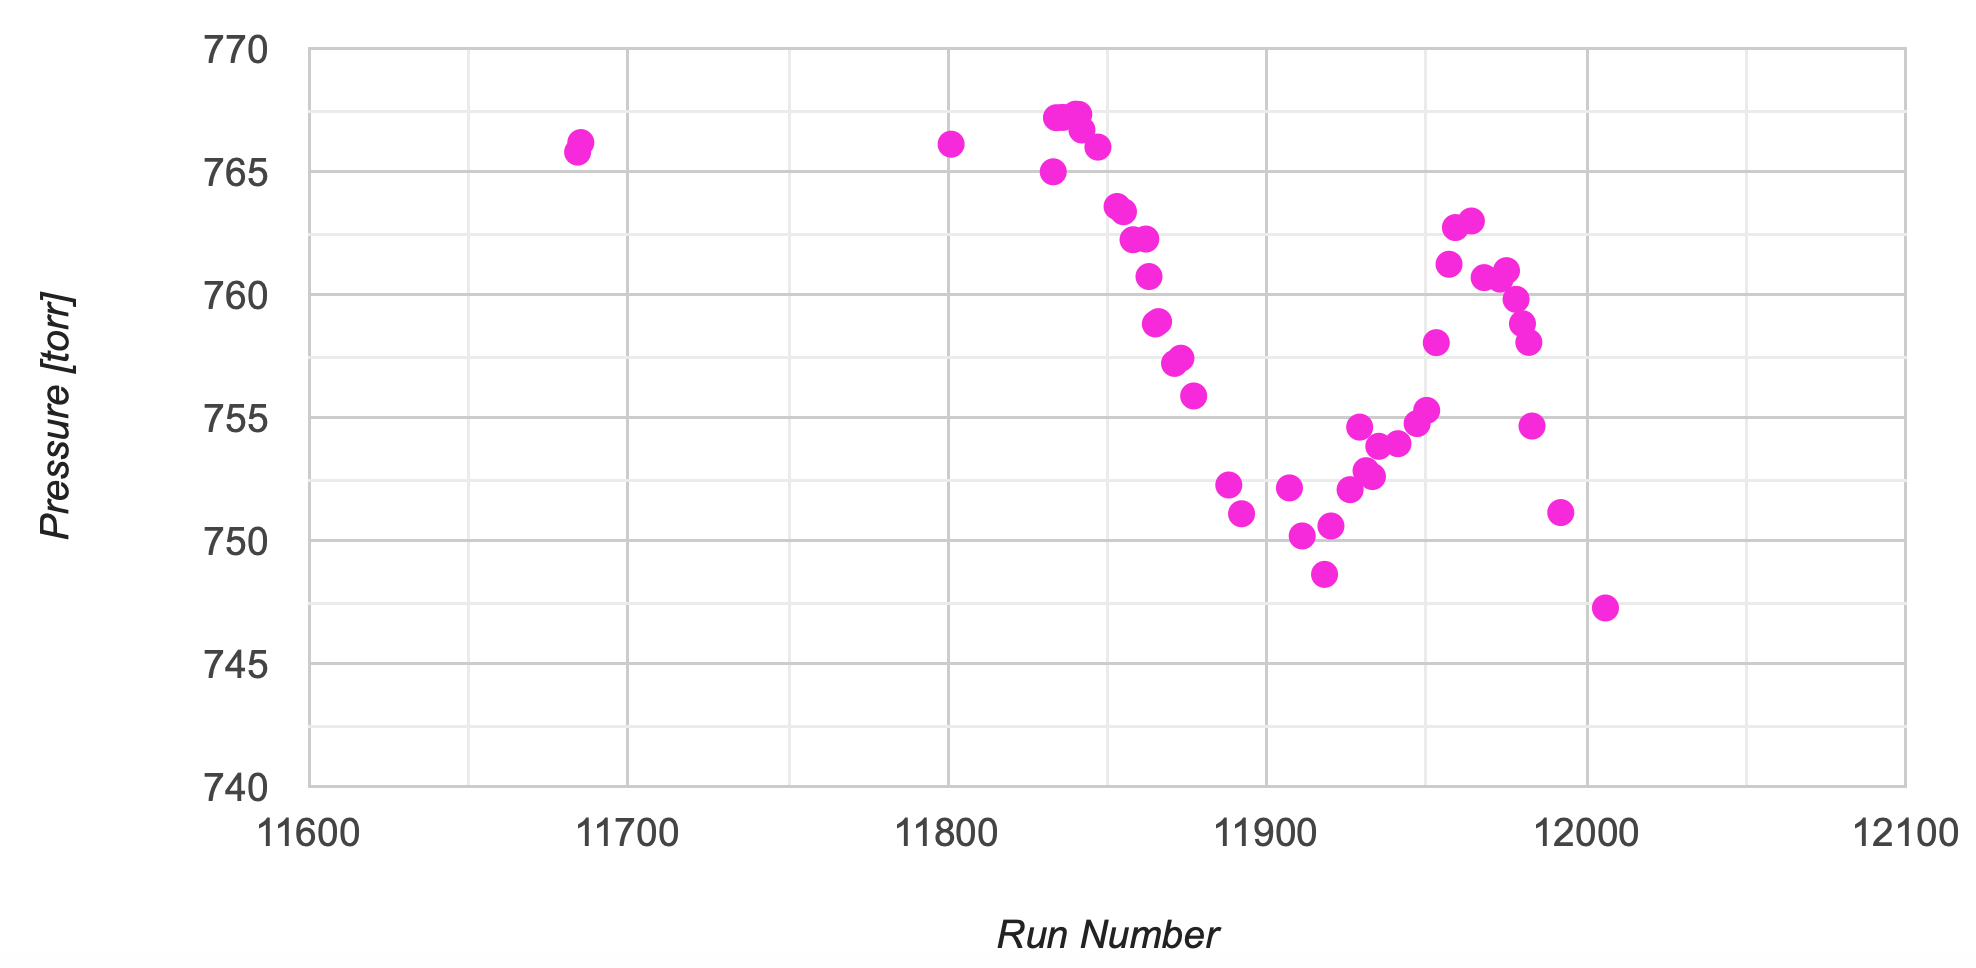
\includegraphics[width=0.9\linewidth]{figures/DMS_pres_run.png}
	\caption{DMS gas pressure vs. run.}
	\label{fig:dms_pres_run}
\end{figure}

The other reason for deviations from typical DMS output was, of course, variations in the parameters it was designed to monitor. When the ambient pressure decreased, the drift times for each channel would decrease, which meant the drift velocity increased. Fig. \ref{fig:dms_ch1_run} shows the channel 1 drift time for each run. Fig. \ref{fig:dms_ch2_run} shows the channel 2 drift time for each run, and Fig. \ref{fig:dms_pres_run} shows the DMS pressure for each run. The ambient pressure began to decrease around Run 11847 to a minimum at Run 11918. This corresponds to the decreased drift times visible during the same runs (Figs. \ref{fig:dms_ch1_run} and \ref{fig:dms_ch2_run}), which means that the DMS was sensitive to changes in gas pressure. Fig. \ref{fig:dms_vel_run} shows the drift velocity over Run Group F.
 
\begin{figure}[h!]
	\centering
	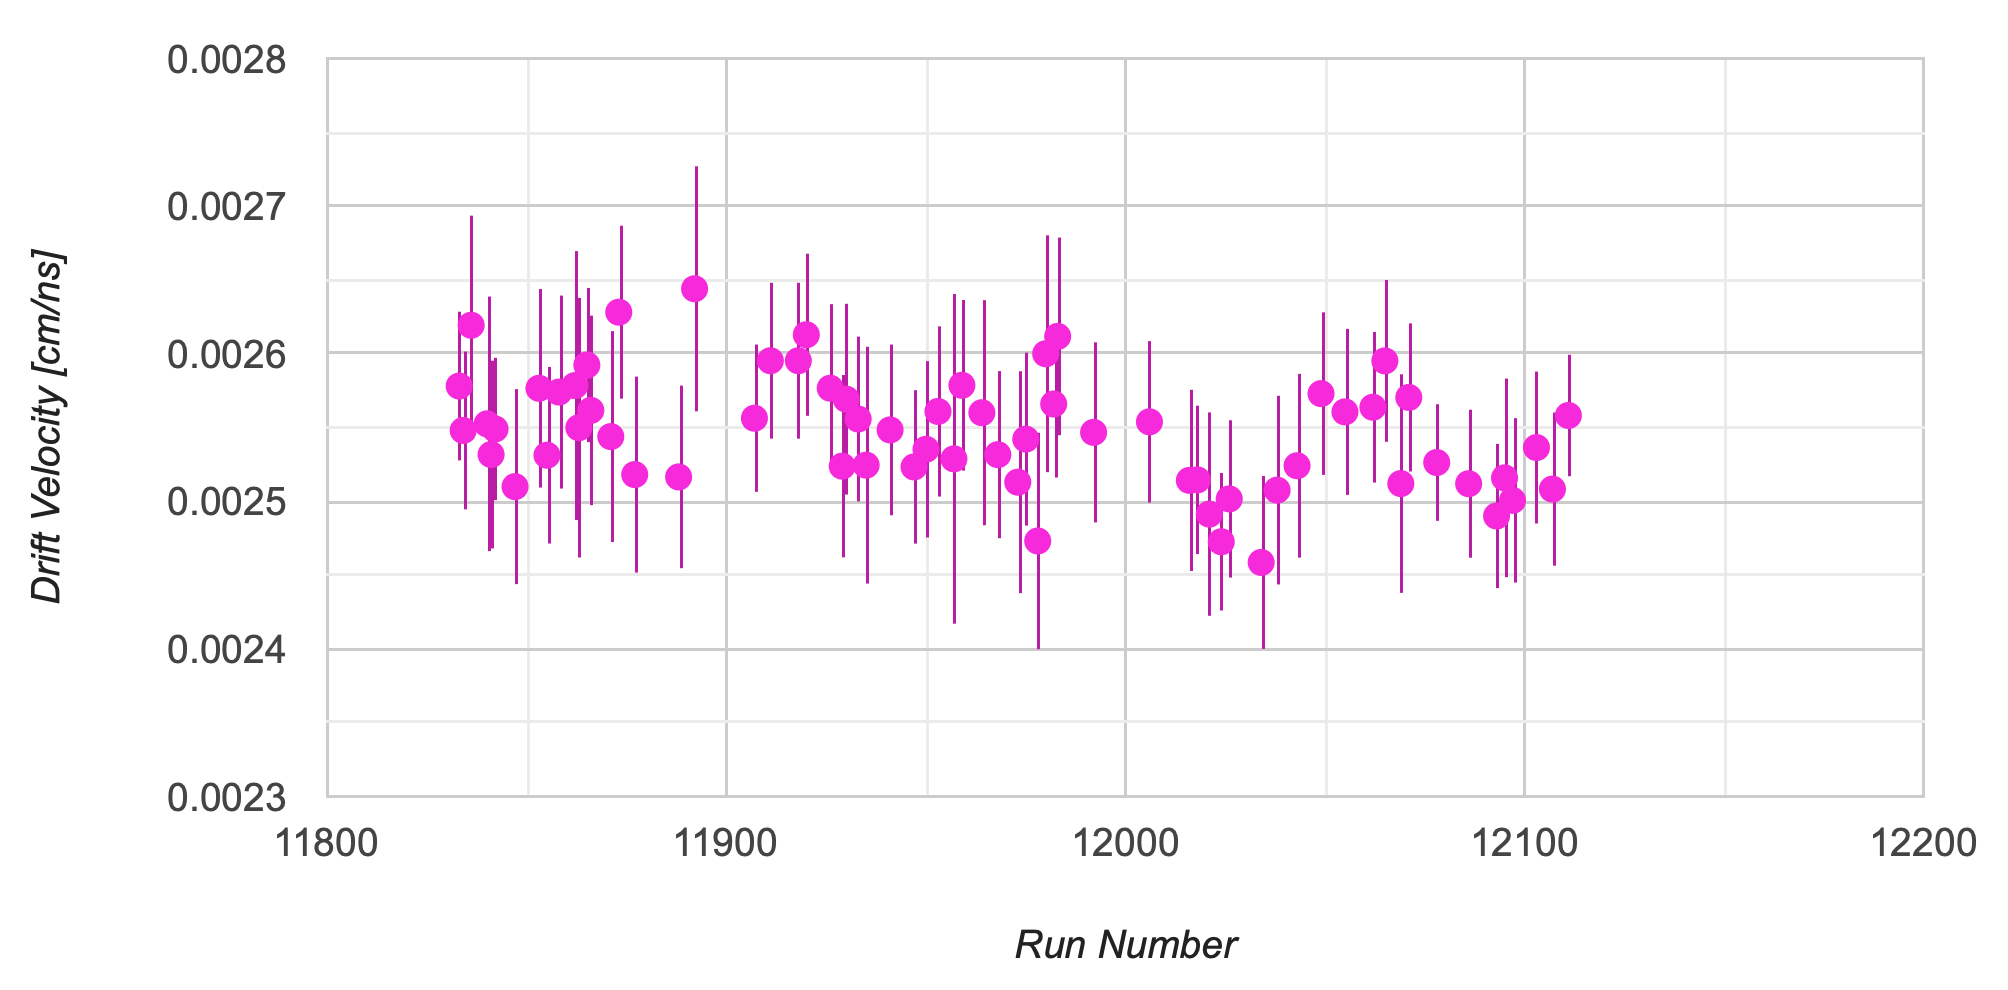
\includegraphics[width=0.9\linewidth]{figures/DMS_vel_run.png}
	\caption{DMS drift velocity over all RGF runs.}
	\label{fig:dms_vel_run}
\end{figure}

\newpage
\subsection{RTPC}
The tracking software developed by David Payette for RTPC hit reconstruction was put into use on RGF data as soon as data started flowing into the DAQ. Fig. \ref{fig:rtpc_tracks_11637} shows two examples of reconstructed tracks using Version 27 of the reconstruction software for Run 11637, which is a 2.14 GeV run at 5 nA. Fig. \ref{fig:rtpc_tracks_12240} shows the reconstructed tracks for separate two time windows in Run 12240, which is a 10.4 GeV run at 240 nA. The increase in current is the reason there are more tracks per event.

\begin{figure}[h!]
	\centering
	\begin{subfigure}[b]{0.44\linewidth}
		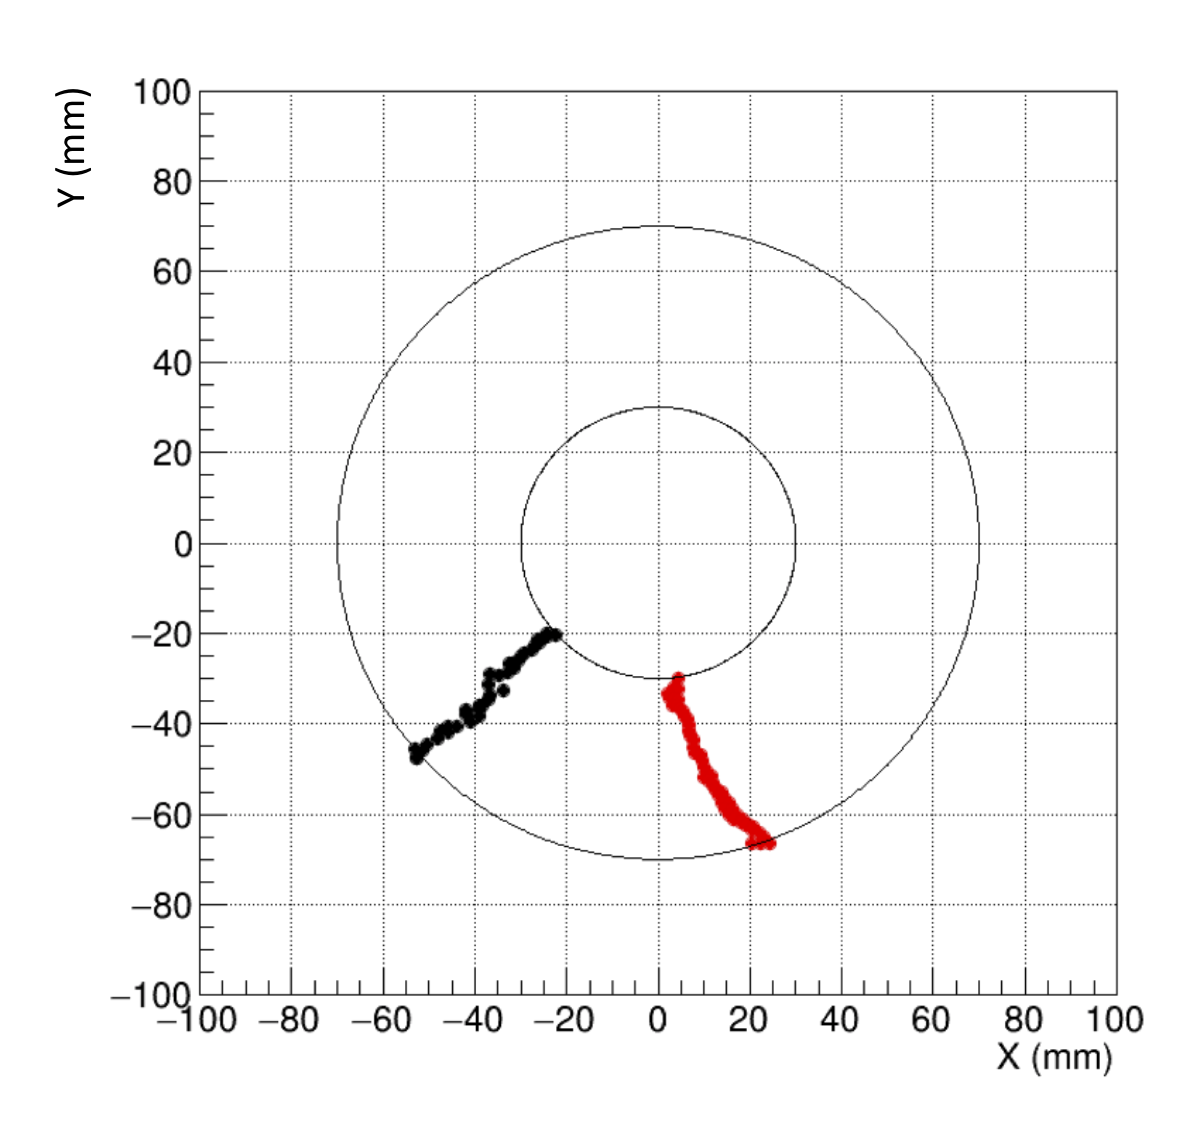
\includegraphics[width=\linewidth]{figures/RTPC_tracks_11637_1.png}
	\end{subfigure}
	\begin{subfigure}[b]{0.44\textwidth}
		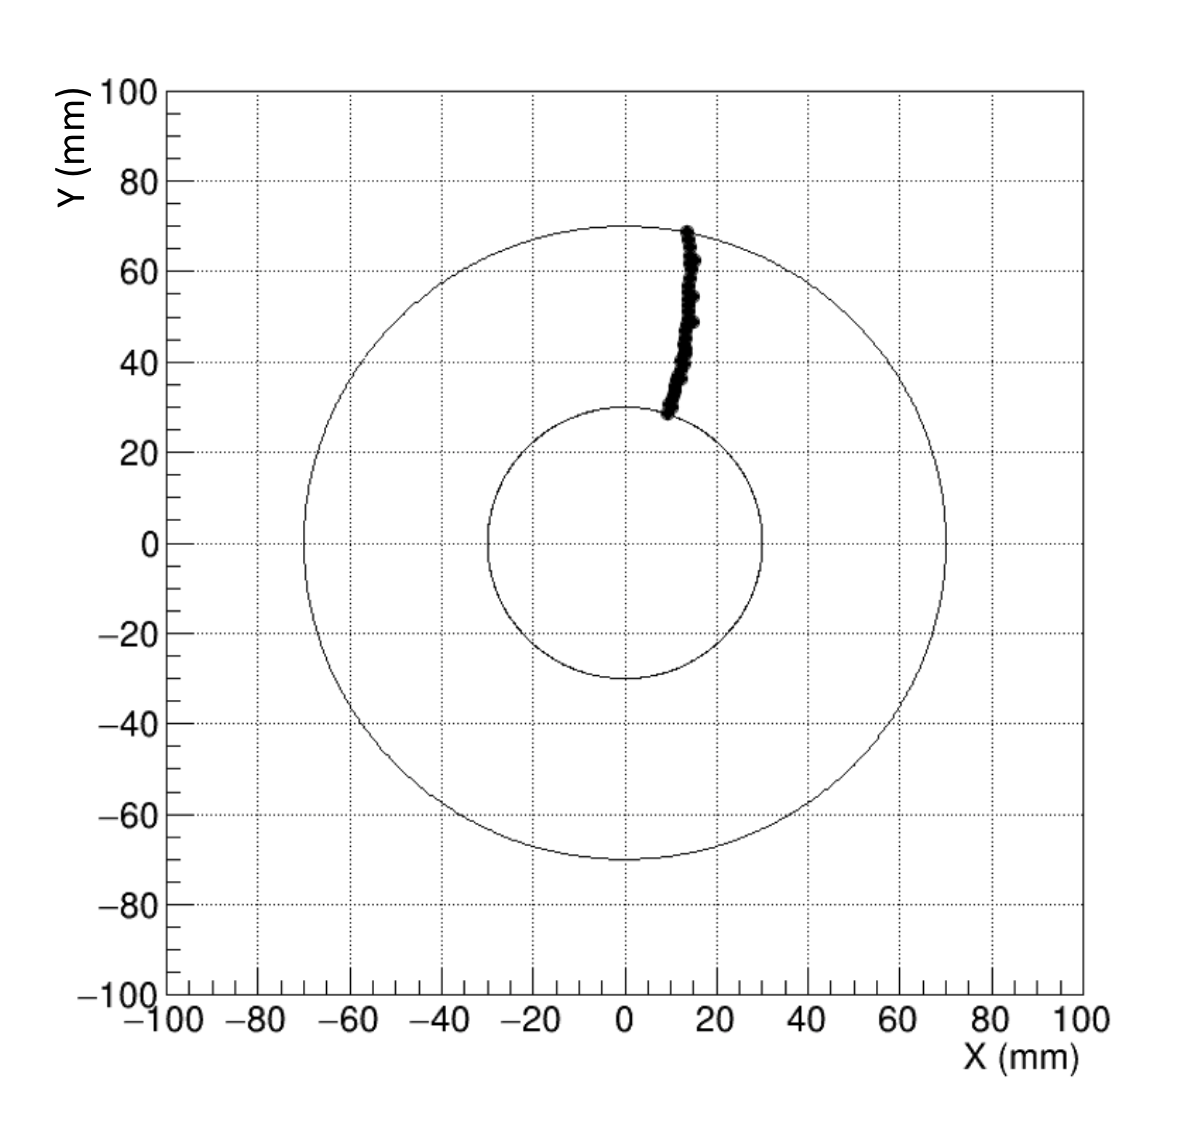
\includegraphics[width=\linewidth]{figures/RTPC_tracks_11637_2.png}
	\end{subfigure}
	\caption{Two examples of reconstructed tracks in one time window in the RTPC using Version 27 of the reconstruction software in a Cartesian $x,y$ space for Run 11637 (2.14 GeV). [\textit{Courtesy D. Payette.}]}
	\label{fig:rtpc_tracks_11637}
\end{figure}
\begin{figure}[h!]
	\centering
	\begin{subfigure}[b]{0.44\linewidth}
		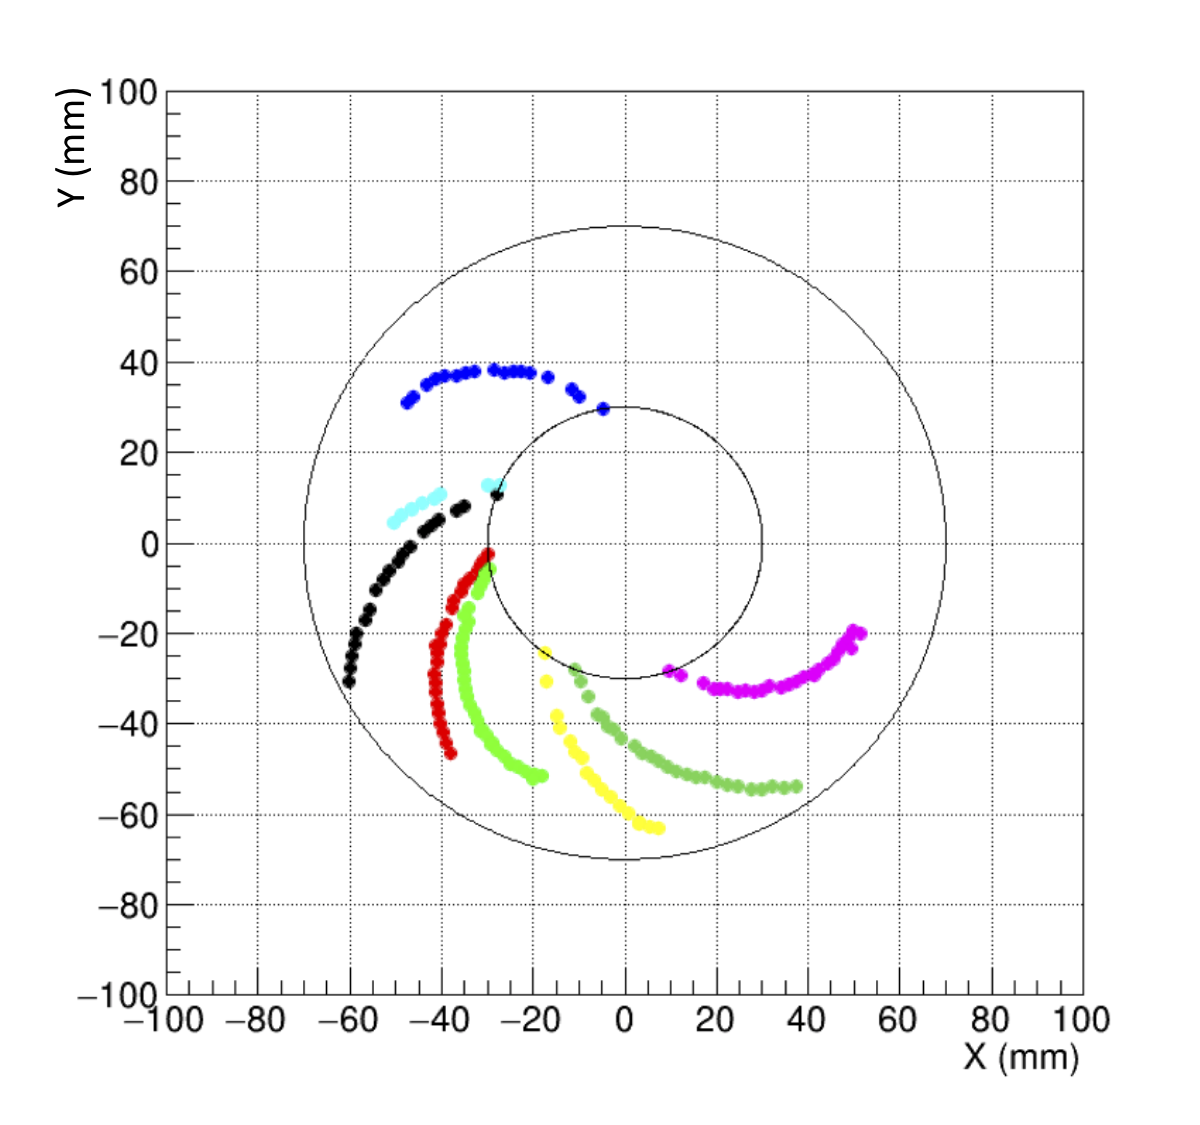
\includegraphics[width=\linewidth]{figures/RTPC_tracks_12240_1.png}
	\end{subfigure}
	\begin{subfigure}[b]{0.44\textwidth}
		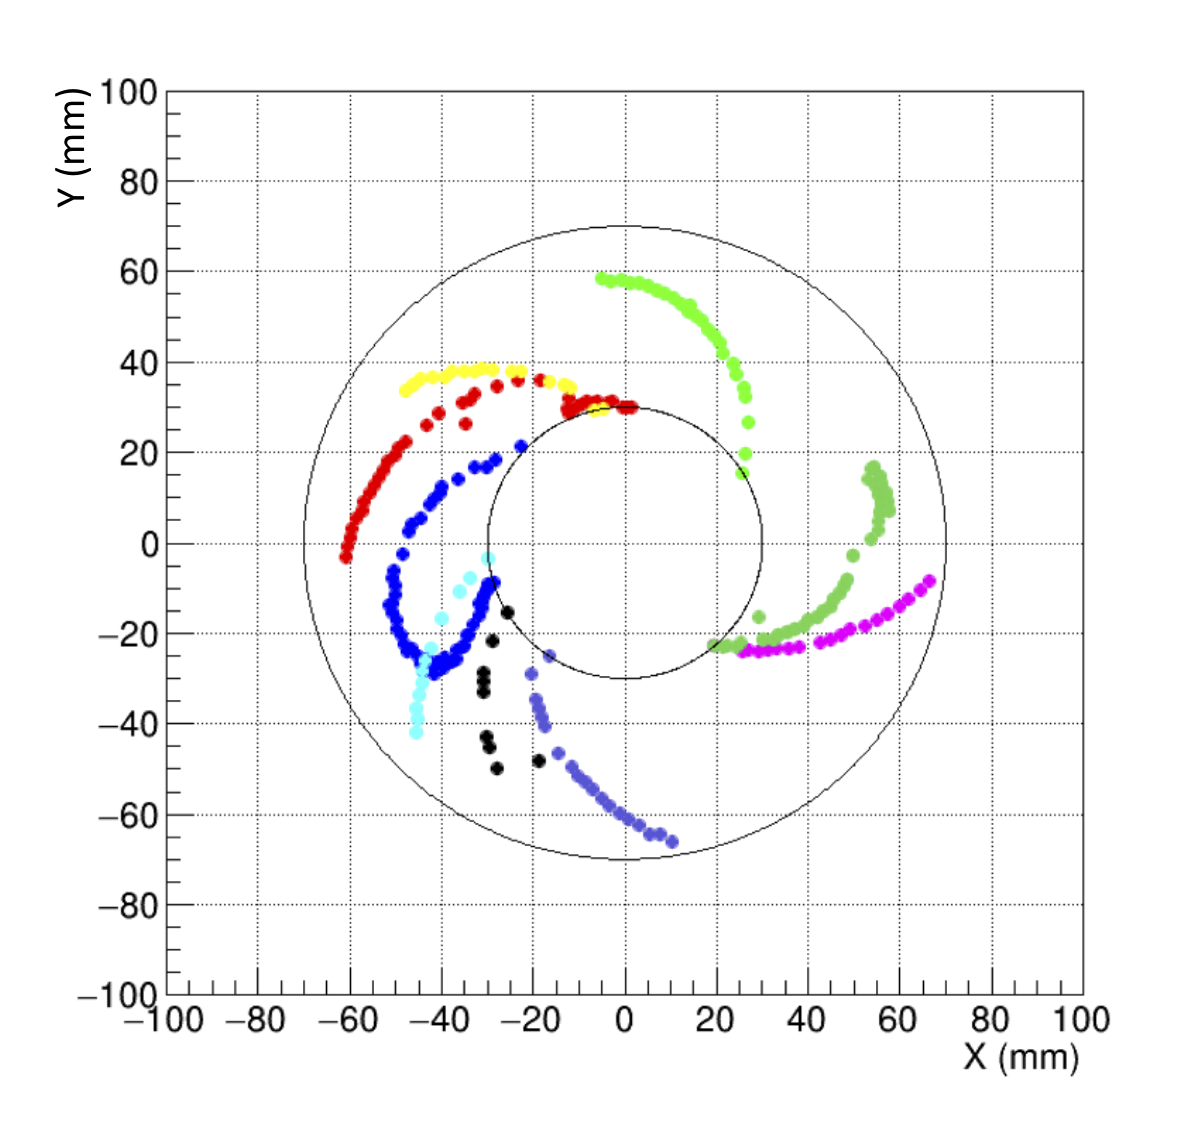
\includegraphics[width=\linewidth]{figures/RTPC_tracks_12240_2.png}
	\end{subfigure}
	\caption{Two examples of reconstructed tracks in one time window in the RTPC using Version 26 of the reconstruction software in an Cartesian $x,y$ space for Run 12240 (10.4 GeV). [\textit{Courtesy D. Payette.}]}
	\label{fig:rtpc_tracks_12240}
\end{figure}

The RTPC reconstruction class, which is integrated into CLARA, consists of a few steps necessary for proton momentum reconstruction that is critical for extraction of the $F_2^n/F_2^p$ structure function ratio. The first is the reconstruction of all hits in an event. This is done using a combination of parameters extracted from Garfield++ and data. The next step is to separate the hits into tracks and disentangle crossing tracks from one another. Finally, once tracks are identified, a helix fitter is used to recover the momentum and vertex of the track. A particle with charge $q$ follows a helical path in a uniform magnetic field $B$ with a certain radius $R$. The momentum of that particle is then
\begin{equation}
p = RqB.
\end{equation}
Obviously, since the magnetic field is not uniform, the charged particle (in our case, the proton) does not travel in an exact helix. The answer to this problem is called a Kalman Filter. The Kalman Filter accounts for non-uniform magnetic fields and decreasing proton momentum by accounting for variations in each step. Implementation of the Kalman Filter will likely be done at a later date.

Once the kinematics of the proton tracks are reconstructed from the raw data, that reconstructed data is analyzed to find the ``good" proton (corresponding to the electron that triggered the event) among the background. This identification in parallel with revisions to the reconstruction code will be an ongoing process. Fig. \ref{fig:rgf_pkin} shows some of the kinematics of the reconstructed protons with one cut on $t_{\mathrm{shift}}$, which is a variable determined from the electron trigger. This cut of $-200 \mathrm{ns} < t_{\mathrm{shift}} < 500 \mathrm{ns}$ is done in an attempt to isolate protons tracks that occur around the time of an identified electron trigger in the CLAS12 forward detectors (FD).

\begin{figure}[h!]
	\centering
	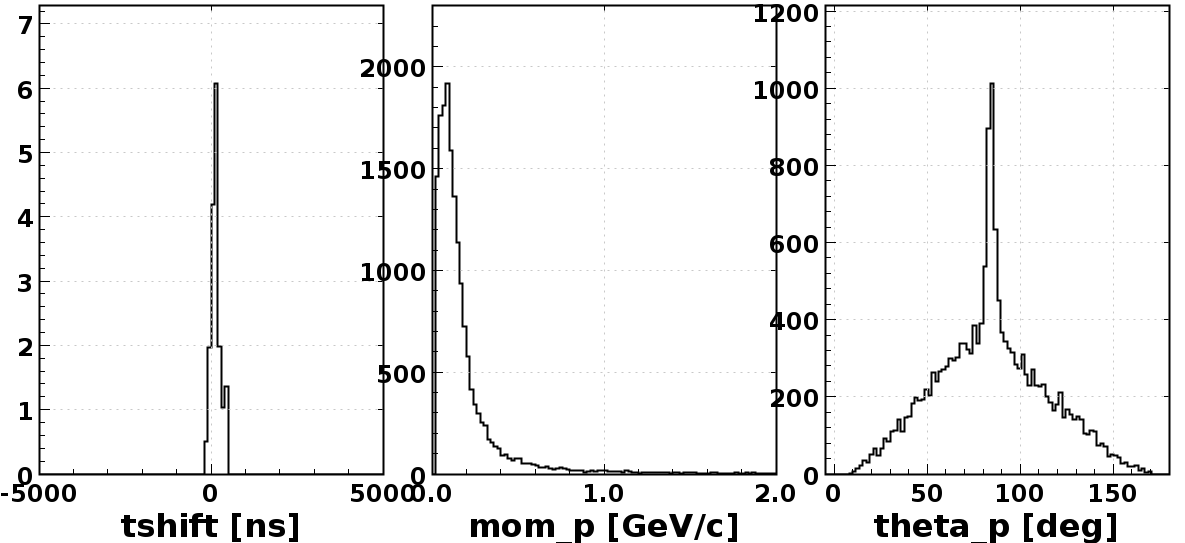
\includegraphics[width=0.9\linewidth]{figures/rgf/11637/pkinematics.png}
	\caption{The time shift ($t_{\mathrm{shift}}$), momentum, and theta ($\theta$) of the reconstructed protons in Run 11637.}
	\label{fig:rgf_pkin}
\end{figure}

Because Run 11637 was a low energy run at 2.14 GeV, it was analyzed in comparison to expected elastic scattering kinematics. For elastic $ep\rightarrow e'p'$ events, the proton momentum is
\begin{equation}
p_{\mathrm{calc}} = \sqrt{Q^2+\frac{Q^4}{4M_P^2}}
\end{equation}
and the scattering angle is
\begin{equation}
\theta_{\mathrm{calc}} = \tan^{-1} \left[ \frac{1}{ \left( 1+\frac{E}{M_p} \right) \tan \left( \frac{\theta_e}{2} \right) } \right],
\end{equation}
where $E$ is the beam energy and $\theta_e$ is the scattering angle of the electron. Fig. \ref{fig:rgf_pmom} shows the 2D distribution of the calculated momentum (``mom\_predicted" in the plot) and measured momentum for protons as well as the difference between the predicted and measured values of the momentum for Run 11637. Fig. \ref{fig:rgf_ptheta} shows the 2D distributions of the calculated theta (``theta\_predicted" in the plot) and measured theta for protons as well as the difference between the predicted and measured values of theta for Run 11637. 

\begin{figure}[h!]
	\centering
	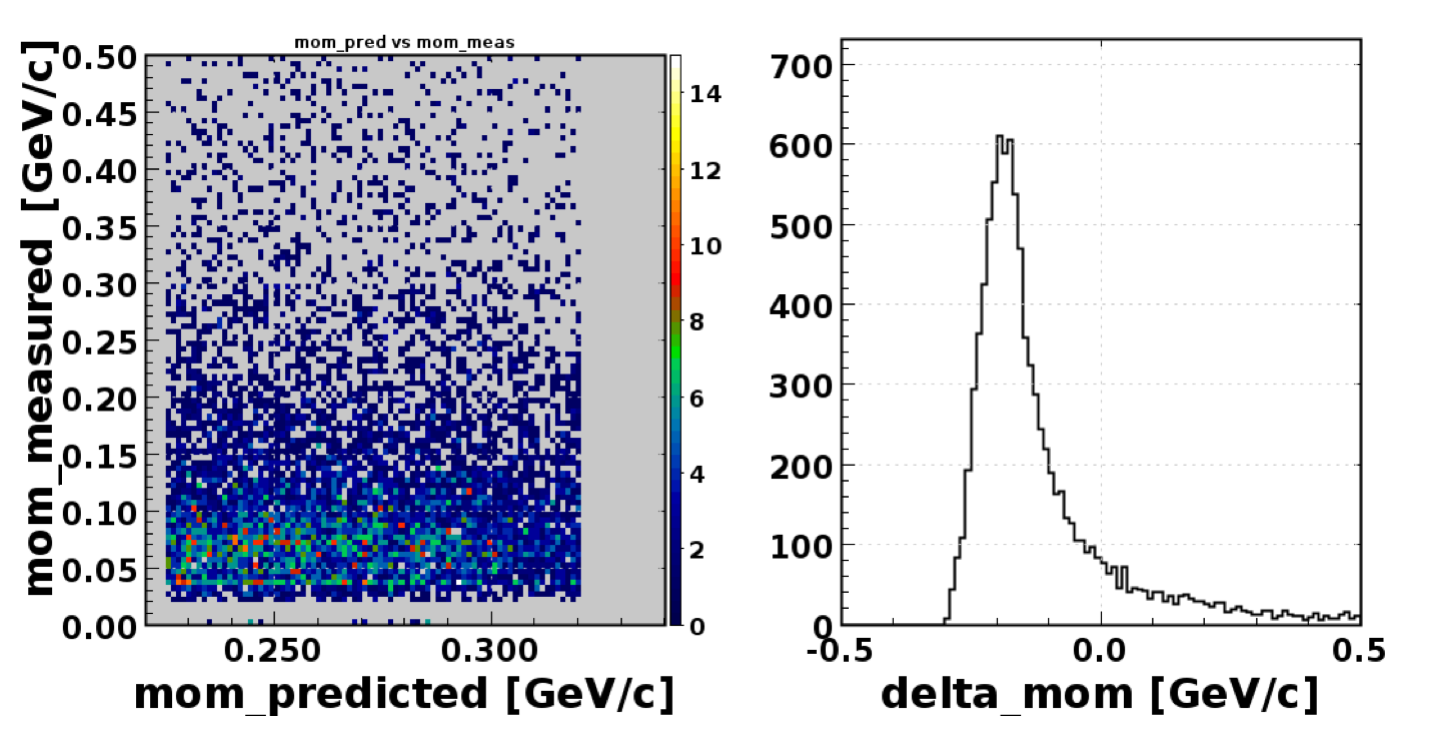
\includegraphics[width=0.9\linewidth]{figures/rgf/11637/momentum.png}
	\caption{On the left: 2D distributions of the calculated momentum (``mom\_predicted" in the plot) on the $x$-axis and reconstructed momentum (``mom\_measured" in the plot) for protons on the $y$-axis in Run 11637. On the right: The difference between the predicted and measured values of the momentum for Run 11637.}
	\label{fig:rgf_pmom}
\end{figure}
\begin{figure}[h!]
	\centering
	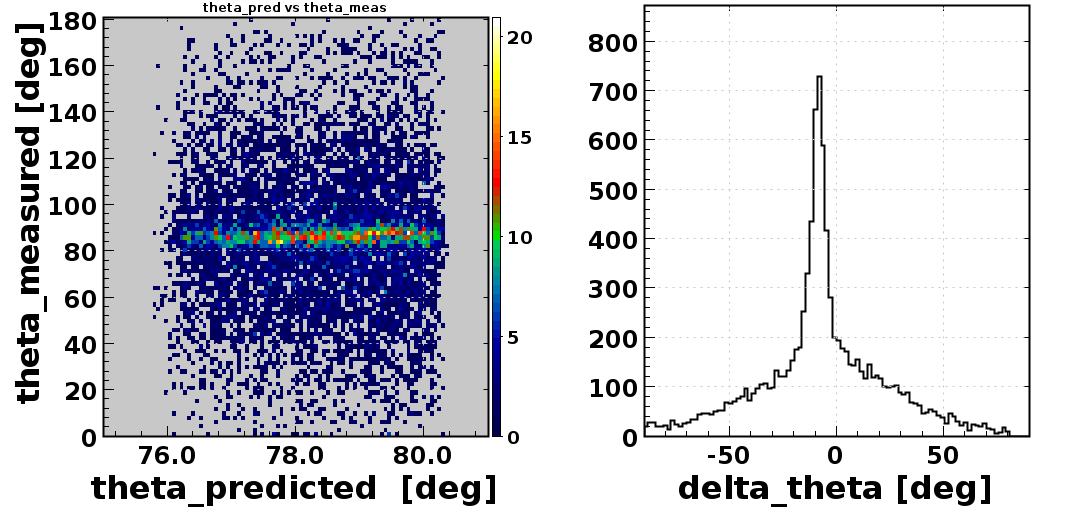
\includegraphics[width=0.9\linewidth]{figures/rgf/11637/ptheta.png}
	\caption{On the left: 2D distributions of the calculated theta (``theta\_predicted" in the plot) on the $x$-axis and reconstructed theta (``theta\_measured" in the plot) for protons on the $y$-axis in Run 11637. On the right: The difference between the predicted and measured values of theta for Run 11637.}
	\label{fig:rgf_ptheta}
\end{figure}

There are some clear irregularities in the reconstruction of proton kinematics. For example, in Fig. \ref{fig:rgf_pmom}, the peak of $\Delta p$ is around 200 MeV, which should be at zero. Calibrations that focus on recovering accurate kinematics will be ongoing by BONuS12 collaborators until expected results for the calibration runs are achieved. Once acceptable calibration occurs, intensive data analysis to recover the proton momentum will begin and likely continue for years to come. This analysis will lead to an extraction of the $F_2^n/F_2^p$ structure function ratio at higher $x$ than previously accessed. Knowing this structure function ratio allows us to know more about the overall structure of the neutron, which was the goal of the simulation and development of the Radial Time Projection Chamber for the Barely Off-shell Nucleon Structure experiment at 12 GeV.

\newpage
\section{Conclusions}
The Drift-gas Monitoring System for the BONuS12 experiment worked well during the experimental run and proved its usefulness in monitoring gas properties. The BONuS12 experiment itself, while it ended rather abruptly, did successfully run for 33 days and gathered 2.8 billion triggers with the RTPC. At this time, calibration of the RTPC is not complete and so the proton kinematics fo not yet agree with elastic scattering predictions. The data gathered will shed light on the the $F_2^n/F_2^p$ ratio, which is the key quantity for understanding the quark structure of the neutron. Extracting this ratio depends on an accurate understanding of the scattered electron as detected in CLAS12. Inclusive deep inelastic scattering from an earlier data set were presented and compared to an established model. The results presented in this work were consistent with previous data, although deviations were observed at small $x$, where the acceptance was considerably small and possibly inaccurate. The overall program of investigating nucleon structure will continue for years to come at Jefferson Lab and then with the Electron Ion Collider at Brookhaven National Lab in Upton, NY.